% Options for packages loaded elsewhere
\PassOptionsToPackage{unicode}{hyperref}
\PassOptionsToPackage{hyphens}{url}
\documentclass[
]{article}
\usepackage{xcolor}
\usepackage{amsmath,amssymb}
\setcounter{secnumdepth}{-\maxdimen} % remove section numbering
\usepackage{iftex}
\ifPDFTeX
  \usepackage[T1]{fontenc}
  \usepackage[utf8]{inputenc}
  \usepackage{textcomp} % provide euro and other symbols
\else % if luatex or xetex
  \usepackage{unicode-math} % this also loads fontspec
  \defaultfontfeatures{Scale=MatchLowercase}
  \defaultfontfeatures[\rmfamily]{Ligatures=TeX,Scale=1}
\fi
\usepackage{lmodern}
\ifPDFTeX\else
  % xetex/luatex font selection
\fi
% Use upquote if available, for straight quotes in verbatim environments
\IfFileExists{upquote.sty}{\usepackage{upquote}}{}
\IfFileExists{microtype.sty}{% use microtype if available
  \usepackage[]{microtype}
  \UseMicrotypeSet[protrusion]{basicmath} % disable protrusion for tt fonts
}{}
\makeatletter
\@ifundefined{KOMAClassName}{% if non-KOMA class
  \IfFileExists{parskip.sty}{%
    \usepackage{parskip}
  }{% else
    \setlength{\parindent}{0pt}
    \setlength{\parskip}{6pt plus 2pt minus 1pt}}
}{% if KOMA class
  \KOMAoptions{parskip=half}}
\makeatother
\usepackage{graphicx}
\makeatletter
\newsavebox\pandoc@box
\newcommand*\pandocbounded[1]{% scales image to fit in text height/width
  \sbox\pandoc@box{#1}%
  \Gscale@div\@tempa{\textheight}{\dimexpr\ht\pandoc@box+\dp\pandoc@box\relax}%
  \Gscale@div\@tempb{\linewidth}{\wd\pandoc@box}%
  \ifdim\@tempb\p@<\@tempa\p@\let\@tempa\@tempb\fi% select the smaller of both
  \ifdim\@tempa\p@<\p@\scalebox{\@tempa}{\usebox\pandoc@box}%
  \else\usebox{\pandoc@box}%
  \fi%
}
% Set default figure placement to htbp
\def\fps@figure{htbp}
\makeatother
\setlength{\emergencystretch}{3em} % prevent overfull lines
\providecommand{\tightlist}{%
  \setlength{\itemsep}{0pt}\setlength{\parskip}{0pt}}
\usepackage{bookmark}
\IfFileExists{xurl.sty}{\usepackage{xurl}}{} % add URL line breaks if available
\urlstyle{same}
\hypersetup{
  hidelinks,
  pdfcreator={LaTeX via pandoc}}

\author{}
\date{}

\begin{document}

{Vue Advance}

\section{\texorpdfstring{{Computed
Properties}}{Computed Properties}}\label{h.70dm3oerka11}

\begin{itemize}
\tightlist
\item
  {Assumono valori dinamici in base ad altre property del nostro oggetto
  Vue;}
\item
  {Possono essere utilizzate come normali proprietà del campo data;}
\end{itemize}

{}

{Usare le computed properties conviene perché usa la }{cache}{, e i
nuovi valori vengono calcolati solo se e quando le dipendenze dovessero
cambiare.}

{Utilizzare le computed piuttosto che i metodi, evita di generare i
valori di ritorno ad ogni accesso, così da }{rigenerarli}{~solo se e
quando le dipendenze dovessero cambiare (}{caching}{).}

{}

{Vengono utilizzate per calcolare il valore di una proprietà in base ad
alcune altre condizioni.}

\section{\texorpdfstring{{Watchers}}{Watchers}}\label{h.bfp2o09kg6gj}

{Si può usare questa opzione per attivare una funzione ogni volta che
una proprietà cambia.}

{}

{\pandocbounded{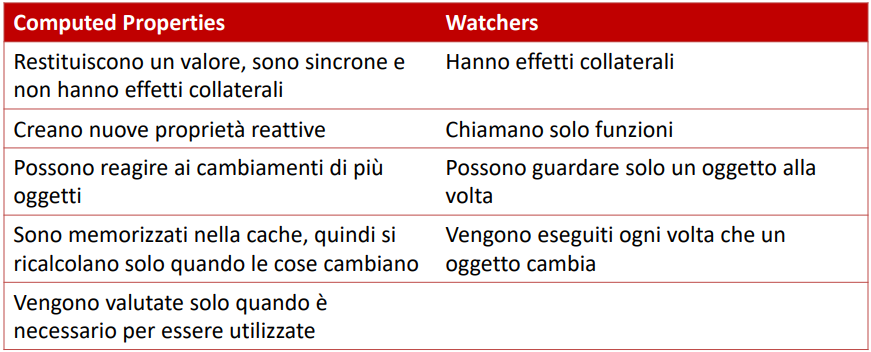
\includegraphics[keepaspectratio]{images/image8.png}}}

\section{\texorpdfstring{{Componenti}}{Componenti}}\label{h.1l868c6wk71g}

{I componenti ci consentono di suddividere l\textquotesingle interfaccia
utente in parti indipendenti e riutilizzabili e di pensare a ogni parte
isolatamente, per farlo possiamo:}

\begin{itemize}
\tightlist
\item
  {utilizzando un custom tag: }{\textless hello-world}{~/\textgreater{}}
\item
  {utilizzando il tag component e l'attributo is: }{\textless component
  :is=''HelloWorld'' /\textgreater{}}
\end{itemize}

{}

{Possiamo registrarli:}

\begin{itemize}
\tightlist
\item
  {Globalmente}{: ma ciò impedisce di rimuovere i componenti
  inutilizzati e rende le relazioni di dipendenza meno esplicite.}
\item
  {Localmente}{: rende disponibile il componente solo
  all\textquotesingle interno del componente in cui è registrato }
\end{itemize}

\section{\texorpdfstring{{Props}}{Props}}\label{h.5livhfyz3iqt}

{Rappresentano attributi custom che permettono di configurare un
componente dall\textquotesingle esterno, definite a priori, è possibile
definire il loro tipo o l'eventualità.}

{}

{Passate ad un componente in maniera statica o dinamica.}

{}

{Vue implementa il cosiddetto }{one-way data flow}{, le prop passate ad
un componente possono essere modificate dall'esterno, ma non dal
componente stesso, in quanto il flusso di dati è
}{monodirezionale,}{~dall'alto al basso.}

{Risolvibile grazie agli eventi custom, è possibile per un componente
comunicare informazioni verso l\textquotesingle esterno, con
l\textquotesingle opzione }{emits}{~un componente può definire a priori
gli eventi che è in grado di emettere e generare eventi.}

{}

{Il cosiddetto }{Prop Drilling}{~è quando dobbiamo passare una prop da
un componente A ad uno C e per farlo lo passiamo a B che è in mezzo.}

{Possiamo evitarlo con il }{Provide - Inject}{, dove A usa
l\textquotesingle opzione }{provide}{~}{per fornire dati a tutti i suoi
discendenti e C usa }{inject }{per ottenere dati forniti tramite provide
da qualsiasi componente ascendente e utilizzarli come normali
properties.}

{}

{Nel progetto abbiamo preferito usare gli eventbus perché i componenti
non hanno una gerarchia diretta.}

\section{\texorpdfstring{{Slots}}{Slots}}\label{h.gml9z0xfadm1}

{Come le props ma per passare codice HTML fra componenti.}

\section{\texorpdfstring{{Composition
API}}{Composition API}}\label{h.xau8iclcatpq}

{Usate al posto delle }{Options API}{~(dividendo il codice nei blocchi
data, computed, methods, ecc.). I blocchi data, computed e methods sono
stati rimpiazzati dalla funzione setup(), che restituisce un oggetto
contenente tutte le variabili a cui il template deve avere accesso,
esiste ref che è grossomodo un equivalente di data.}

{}

{Rispetto alle }{options}{~API c'è maggior libertà
nell\textquotesingle organizzazione del codice, miglior supporto a
TypeScript e codice più compatto.}

{}

{Aggiungendo l\textquotesingle attributo setup al tag
\textless script\textgreater{} il contenuto del tag diventi quello della
funzione setup().}

{}

{}

{Node.js}

{Una piattaforma software cross-platform che permette di creare il
proprio Web server.}

{}

{Web application con connessioni real-time, two-way, dove non solo il
client, ma anche il server può iniziare una connessione, permettendo di
trasferire dati liberamente.}

{Usa un modello I/O non bloccante e ad eventi, che lo rende un framework
leggero ed efficiente, le richieste vengono tradotte in eventi (ognuno
dei quali è associato a un event handler) e inserite in una coda. C'è un
event loop single-threaded che controlla se ci sono nuovi eventi nella
coda.}

{}

{Node.js è capace di gestire un elevato numero di connessioni
simultanee. Non congeniale per applicazioni CPU-intensive.}

{}

{Node.js incorpora Node Package Manager (NPM), il più grande ecosistema
di librerie open source al mondo.}

{}

{}

{PHP}

{PHP è un linguaggio di scripting, interpretato, originariamente
concepito per la programmazione di pagine Web dinamiche lato server.}

{}

{L'interprete }{PHP pre processa}{~tutti i file con estensione PHP, che
sono sostanzialmente file contenenti HTML, all'interno dei quali è
presente del codice PHP, contenuto all'interno dei delimitatori
}{\textless?php \ldots{} ?\textgreater{}}{. Ma è possibile anche creare
file con estensione }{.php}{~per poi }{includerli}{~nel file
principale.}

{}

{La sintassi PHP è di tipo C-like:}

{\pandocbounded{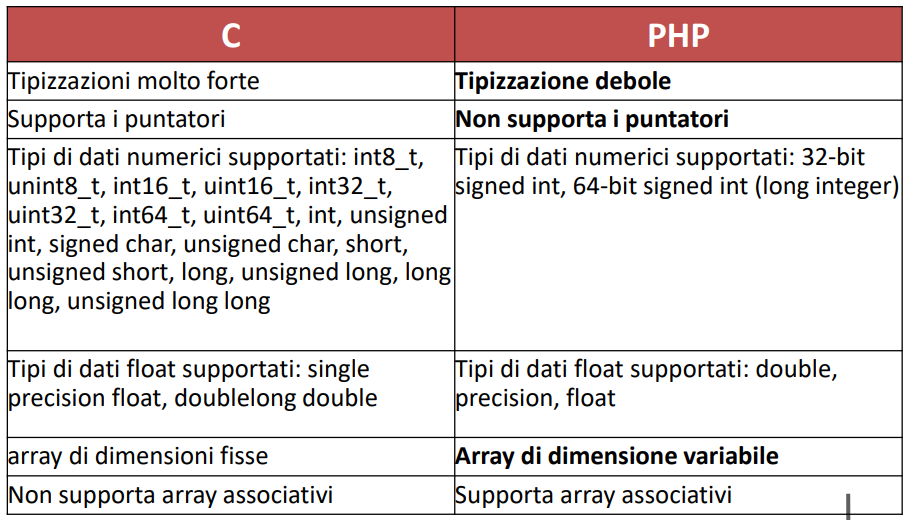
\includegraphics[keepaspectratio]{images/image1.png}}}

\section{\texorpdfstring{{Cookies}}{Cookies}}\label{h.i13gpae1ysjp}

{Sono un meccanismo di supporto alla gestione delle sessioni basato
sull'idea che sia il client a mantenere lo stato di precedenti
connessioni, e ad inviarlo al server di pertinenza ogni volta che
richiede un documento.}

{}

{Il termine cookie indica un blocco di dati opaco lasciato dal server in
consegna ad un richiedente per poter ristabilire in seguito il suo
diritto alla risorsa richiesta . }

{}

{Alla prima richiesta di uno user-agent, il server fornisce la risposta
ed un header aggiuntivo, il cookie, con dati arbitrari e con la
specifica di usarlo per ogni successiva richiesta. Il server associa a
questi dati le informazioni sulla transazione. Ogni volta che lo
user-agent }{accederà}{~a questo sito, rifornirà i dati opachi del
cookie che permettono al server di ri-identificare il richiedente, e
creare così un profilo specifico. }

\subsection{\texorpdfstring{{Tipi}}{Tipi}}\label{h.8zti3wblacc2}

\begin{itemize}
\tightlist
\item
  {Tecnici}{: usati dal gestore del sito per mettere in opera alcune
  funzioni o rendere più agile la navigazione;}
\item
  {Analitici}{: usati dal gestore del sito per raccogliere alcune
  informazioni in forma aggregata sugli utenti;}
\item
  {Di profilazione}{: sono usati dal gestore del sito per raccogliere
  dati personali sui visitatori {[}solo questi è necessario
  accettare{]}.}
\end{itemize}

{}

{}

{}

{}

{}

{}

{JavaScript Advanced}

\section{\texorpdfstring{{API HTML5}}{API HTML5}}\label{h.7b8tns7uhier}

\subsection{\texorpdfstring{{WebStorage}}{WebStorage}}\label{h.35qskvq49n6o}

{Le API WebStorage consentono di salvare e recuperare dati localmente al
browser, dati memorizzati in coppie chiave-valore.}

{Due oggetti principali:}

\begin{itemize}
\tightlist
\item
  {localStorage}{: i dati non hanno scadenza e non vengono cancellati
  alla chiusura del browser.}
\item
  {sessionStorage}{: a differenza di localStorage, i dati sono mantenuti
  solo per la sessione corrente e cancellati quando il browser viene
  chiuso. }
\end{itemize}

{}

{A differenza dei cookies: }

\begin{itemize}
\tightlist
\item
  {Limite di memoria più ampio 10MB contro i 4MB dei Cookie.}
\item
  {Non ha una data di scadenza.}
\item
  {Non è possibile gestirli lato server.}
\end{itemize}

\subsection{\texorpdfstring{{WebWorker}}{WebWorker}}\label{h.813equ539fxl}

{Permettono di eseguire codice Javascript in background.}

\subsection{\texorpdfstring{{Drag and
Drop}}{Drag and Drop}}\label{h.p8p436ir86kj}

{Le API Drag and Drop consentono di effettuare operazioni di drag and
drop all'interno della pagina.}

\subsection{\texorpdfstring{{Geolocation}}{Geolocation}}\label{h.vpfu1enj2l98}

{L'API Geolocation consente di ottenere la posizione geografica
dell'utente.}

\subsection{\texorpdfstring{{IndexedDB}}{IndexedDB}}\label{h.etene0n9zcjv}

{Le API IndexedDB consentono di creare e manipolare un database
all'interno del browser, consentono di memorizzare quantità di dati
strutturati più }{grande rispetto alle API WebStorage.}{~}

\section{\texorpdfstring{{API
JavaScript}}{API JavaScript}}\label{h.30h83gxlxmt2}

\subsection{\texorpdfstring{{WebSocket}}{WebSocket}}\label{h.uvonku9ta1zw}

{Le WebSocket consentono di instaurare un canale di comunicazione
full-duplex attraverso una singola connessione TCP.}

\subsection{\texorpdfstring{{WebForms}}{WebForms}}\label{h.x5u55blccwvv}

{Sono API per la validazione dei campi di input.}

\subsection{\texorpdfstring{{WebHistory}}{WebHistory}}\label{h.yebyddlkikrw}

{Web History fornisce un accesso facilitato all'oggetto windows.history,
che contiene gli URL visitati dall'utente.}

\section{\texorpdfstring{{ECMAScript}}{ECMAScript}}\label{h.rtfxajinca7g}

{Specifica ~tecnica di un linguaggio di scripting, standardizzata e
mantenuta da ECMA International }{nell\textquotesingle ECMA262}{~ed
ISO/IEC 16262, la sua implementazione più conosciuta è Javascript.}

{}

{Le versioni vanno da }{ES2}{~a }{ES6}{. }

{}

{L'ultima versione aggiunge }{Promise}{~che consente di gestire
l\textquotesingle eventuale completamento, o fallimento, di
un\textquotesingle operazione asincrona.}

{In una promessa, il valore non è necessariamente noto al momento della
creazione e la ~promessa consente di associare handler sia in caso di
successo che di errore di un'operazione asincrona; invece di restituire
il valore in modo sincrono, l'idea è quella di restituire la promessa di
fornire il valore in un momento futuro.}

{\pandocbounded{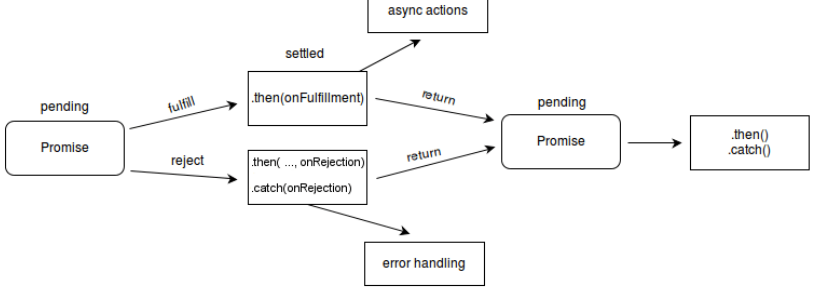
\includegraphics[keepaspectratio]{images/image7.png}}}

{Un'altra aggiunta sono le }{async/await}{, uno zucchero sintattico che
semplifica l'utilizzo delle funzioni asincrone e, di conseguenza, anche
delle Promise.}

{}

{}

{Mobile}

{Alcune definizioni:}

{}

{Consiste in tecniche/tecnologie che permettono a utenti in movimento di
utilizzare device portatili, di eseguire applicazioni e di connettersi
ad applicazioni remote.}

{}

{È una tecnologia che consente la trasmissione di dati, voce e video
tramite un computer o qualsiasi altro dispositivo abilitato wireless
senza dover essere collegato ad un collegamento fisico fisso.}

{}

{È un termine generico che si riferisce a una varietà di dispositivi che
permettono alle persone di accedere a dati e informazioni ovunque si
trovino.}

{}

{Nel mobile bisogna rispettare alcune caratteristiche, come:}

{}

{Portabilità}{: ridurre la dimensione dei dispositivi in modo da creare
computer che potessero essere portati in giro con relativa facilità.}

{}

{Miniaturizzazione}{: creare componenti hardware nuovi e molto piccoli
che permettano l'utilizzo del dispositivo personale durante uno
spostamento.}

{}

{Connettività}{: sviluppare dispositivi e applicazioni che permettessero
all'utente di essere online e di comunicare wireless durante gli
spostamenti.}

{}

{Bluetooth Low Energy (BLE) è una tecnologia di rete personale senza
fili che mira a nuove applicazioni nel settore sanitario, fitness,
beacon (trasmettitori hardware che trasmettono il loro identificatore ai
dispositivi elettronici portatili vicini.), sicurezza e intrattenimento
domestico.}

{}

{Convergenza :}{~integrare tutti i dispositivi esistenti in un unico
dispositivo ibrido in grado di fare tutto.}

{}

{Divergenza}{: ogni dispositivo è pensato per svolgere una specifica
funzione.}

{}

{Altri attori possono essere: }

{Mobile communication}{: infrastruttura creata per garantire una
comunicazione continua e affidabile per lo scambio di dati e voce
utilizzando reti wireless.}

{}

{Hardware mobile}{: dispositivo di elaborazione portatile con la
capacità di recuperare ed elaborare i dati.}

{}

{Software mobile}{: è il programma software che è stato sviluppato
specificamente per essere eseguito su hardware mobile.}

{}

{}

{Alcuni problemi da affrontare nel mobile sono:}

\begin{itemize}
\tightlist
\item
  {I dispositivi mobile sono «resource-constrained».}
\item
  {La connettività mobile è altamente variabile in termini di
  prestazioni e affidabilità.}
\item
  {I dispositivi mobili sono intrinsecamente meno sicuri, inoltre nuove
  problematiche dovute alla privacy.}
\end{itemize}

\section{\texorpdfstring{{Sviluppo
mobile}}{Sviluppo mobile}}\label{h.tyh2meq37x82}

{Conviene scegliere nativo o ibrido? Dipende da:}

\begin{itemize}
\tightlist
\item
  {Che tipo di app deve essere sviluppata;}
\item
  {Esigenze degli utenti.}
\end{itemize}

\subsection{\texorpdfstring{{Native}}{Native}}\label{h.3sg7h1c299nz}

{Applicazioni sviluppate appositamente per un sistema operativo,
utilizzando il suo linguaggio di sviluppo.}

{}

{Vantaggi:}

\begin{itemize}
\tightlist
\item
  {High performance }
\item
  {Sicurezza}
\item
  {Personalizzazione (UX)}
\item
  {Forte compatibilità con altre app}
\item
  {Assoluta compatibilità con API fornite dal OS}
\end{itemize}

{Svantaggi:}

\begin{itemize}
\tightlist
\item
  {Costo}
\item
  {Tempistiche}
\end{itemize}

{\pandocbounded{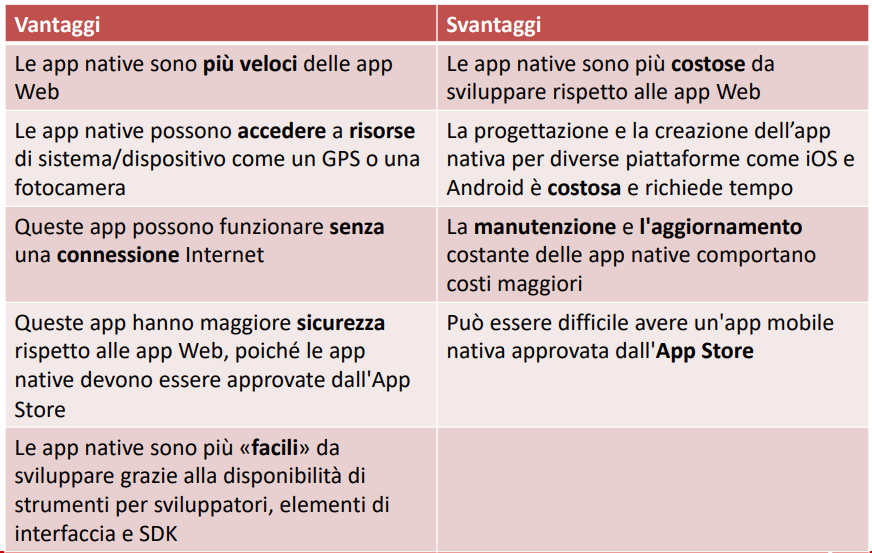
\includegraphics[keepaspectratio]{images/image9.png}}}

\subsection{\texorpdfstring{{(Responsive) Web
app}}{(Responsive) Web app}}\label{h.2z654vqvxfas}

{È possibile accedere alle web app tramite il browser del dispositivo
mobile, non è necessario scaricare e installare l\textquotesingle app su
un dispositivo mobile per usarle, sviluppata come pagine Web e può
essere utilizzata sulla maggior parte dei dispositivi in grado di
navigare sul web.}

{\pandocbounded{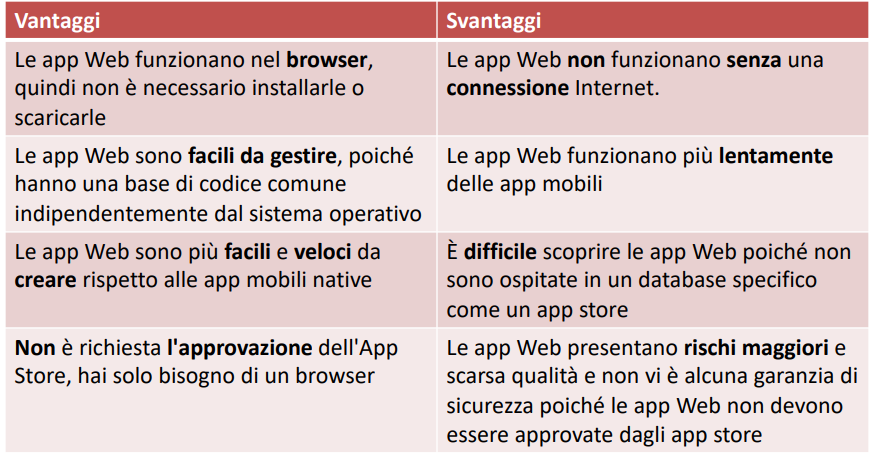
\includegraphics[keepaspectratio]{images/image3.png}}}

{Queste applicazioni Web sono utilizzabili in qualsiasi dimensione del
riquadro di visualizzazione del browser (usabilità).}

\subsection{\texorpdfstring{{Progressive Web
App}}{Progressive Web App}}\label{h.wby8il5jsxta}

{Un\textquotesingle applicazione Web progressiva (PWA) è distribuita
attraverso il Web e creata utilizzando tecnologie web}{.}

{}

{Sono app web che simulano il comportamento delle app mobili native}

{}

{Utilizzano funzionalità della piattaforma Web in combinazione con il
miglioramento progressivo per offrire agli utenti
un\textquotesingle esperienza pari a quella delle app native.}

{}

{Per }{progressively enhanced}{~si intende una strategia nel web design
che pone l\textquotesingle accento sul contenuto, consentendo a tutti di
accedere al contenuto e alle funzionalità di base, mentre gli utenti con
funzionalità del browser aggiuntive o un accesso a Internet più rapido
ricevono la versione avanzata.}

{Questa strategia prevede la separazione del contenuto dalla
presentazione.}

{\pandocbounded{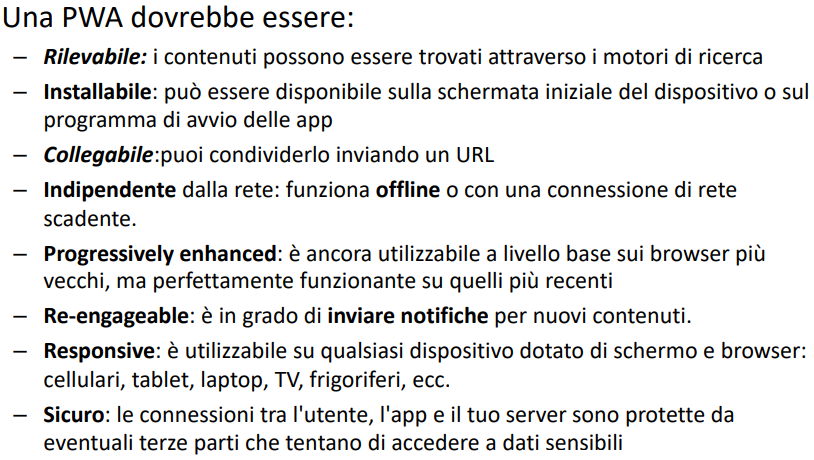
\includegraphics[keepaspectratio]{images/image13.png}}}

{}

\subsection{\texorpdfstring{{Ibrido}}{Ibrido}}\label{h.k0ql7g20mgrv}

{Le app mobili ibride sono applicazioni installate su un dispositivo,
proprio come qualsiasi altra app, ciò che le differenzia è il fatto che
combinano elementi da app native con elementi da app Web.}

{}

{Distribuite in un contenitore nativo che usa un oggetto WebView mobile.
Quando si utilizza l\textquotesingle app, questo oggetto visualizza i
contenuti web grazie all\textquotesingle utilizzo di tecnologie web.}

{}

\section{\texorpdfstring{{Come sviluppare
app}}{Come sviluppare app}}\label{h.akdlf9bawgvg}

{Ecco alcune tecnologie:}

\begin{itemize}
\tightlist
\item
  {Flutter}{: creato da Google, utilizzato per sviluppare applicazioni
  multipiattaforma, usa Dart come linguaggio;}
\item
  {React Native}{: create da Facebook, utilizzato per sviluppare
  applicazioni Android e iOS, usa JavaScript e tecnologie web;}
\item
  {Ionic Framework}{: è un toolkit dell\textquotesingle interfaccia
  utente open source per la creazione di app mobili e desktop
  performanti e di alta qualità utilizzando tecnologie Web, consente di
  creare app per tutti i principali app store da
  un\textquotesingle unica base di codice, nativo e ottimizzato per il
  web;}
\item
  {Cordova}{: framework di sviluppo mobile open source di Apache che
  utilizza le tecnologie web;}
\item
  {Capacitor}{: progetto open source che esegue app Web moderne in modo
  nativo su iOS, Android e Web.}
\end{itemize}

{}

{}

{}

{}

{}

{Data Visualization}

{Quando si usano i dati per mostrare o spiegare qualcosa in maniera
visiva, esempio:}

{\pandocbounded{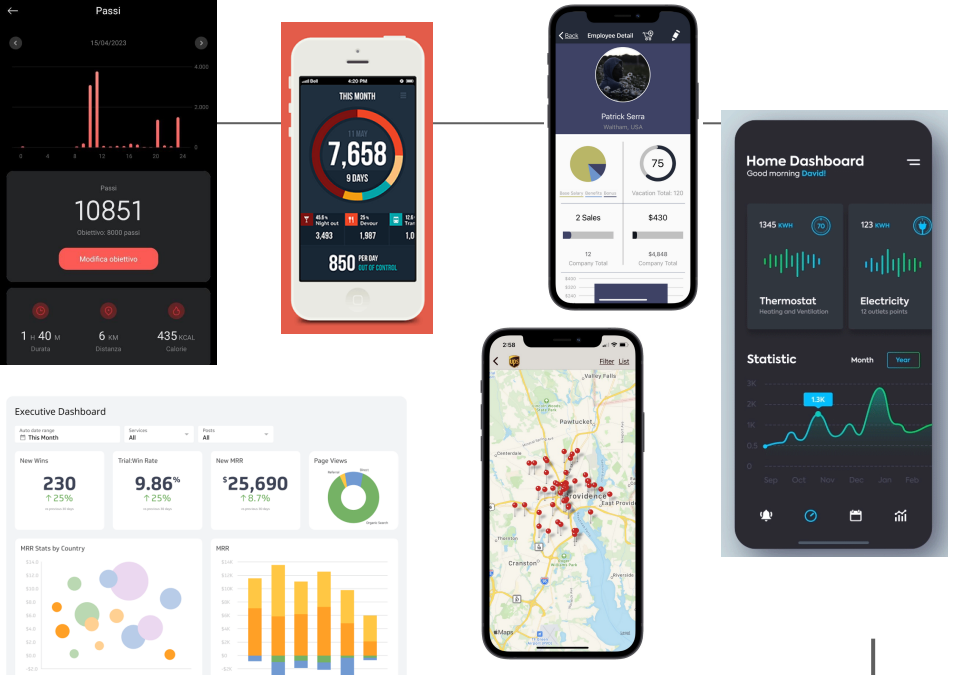
\includegraphics[keepaspectratio]{images/image6.png}}}

{Si usa perchè: l\textquotesingle idea della visualizzazione ci aiuta a
vedere ciò che non abbiamo notato prima. Particolarmente vero quando si
cerca di identificare le relazioni e di trovare un significato in enormi
quantità di dati raccolti (cioè i Big Data).}

{}

{Visualization}{: qualsiasi tipo di rappresentazione visiva di
informazioni progettata per consentire la comunicazione,
l\textquotesingle analisi, la scoperta, l\textquotesingle esplorazione,
la trasmissione di un messaggio, ecc. }

{}

{Information Visualization}{: studio delle rappresentazioni visive di
dati astratti ( sia dati numerici che non numerici) per rafforzare la
cognizione umana. }

{}

{Infografica}{: rappresentazione visiva di informazioni in più sezioni
con lo scopo di comunicare uno o più messaggi specifici. }{Con lo
}{scopo }{di rendere i dati facilmente comprensibili a colpo
d\textquotesingle occhio o con una breve attenzione}{.}

{}

{Data visualization}{: rappresentazione grafica di informazioni e dati.}

{}

\section{\texorpdfstring{{Qualità delle buone
visualizzazioni}{:}}{Qualità delle buone visualizzazioni:}}\label{h.3il1p9ix1qdp}

\begin{enumerate}
\tightlist
\item
  {Truthful}{: }{essere onesti facendo le giuste scelte di design.}
\end{enumerate}

{}

\begin{enumerate}
\setcounter{enumi}{1}
\tightlist
\item
  {Functional}{: }{scegliere le forme grafiche in base ai compiti che si
  desidera permettere di fare.}
\end{enumerate}

{}

\begin{enumerate}
\setcounter{enumi}{2}
\tightlist
\item
  {Beautiful}{: ~gli oggetti devono essere o vissuti come belli dal
  maggior numero possibile di persone.}
\end{enumerate}

{}

\begin{enumerate}
\setcounter{enumi}{3}
\tightlist
\item
  {Insightful}{: le buone visualizzazioni aprono la strada a scoperte
  preziose che sarebbero inaccessibili se le informazioni fossero
  presentate in un modo diverso. }
\end{enumerate}

{}

\begin{enumerate}
\setcounter{enumi}{4}
\tightlist
\item
  {Enlightening}{: qualità composta dalle quattro precedenti.}
\end{enumerate}

{}

\section{\texorpdfstring{{Processo di visualizzazione dei
dati}}{Processo di visualizzazione dei dati}}\label{h.4hks72tugq8f}

{}

{\pandocbounded{
\includegraphics[keepaspectratio]{images/image10.png}}}

{}

{I dati possono essere:}

\begin{itemize}
\tightlist
\item
  {Categorici}{: descrivono categorie o gruppi }
\item
  {Numerici}{: rappresentano numeri (quantità, range ecc..)}
\end{itemize}

{}

{Per la visualizzazione esistono diversi grafici:}

\begin{itemize}
\tightlist
\item
  {Bar chart}{: per comparare più valori, se modifichiamo troppo la
  scala manipoliamo le informazioni.}
\end{itemize}

{\pandocbounded{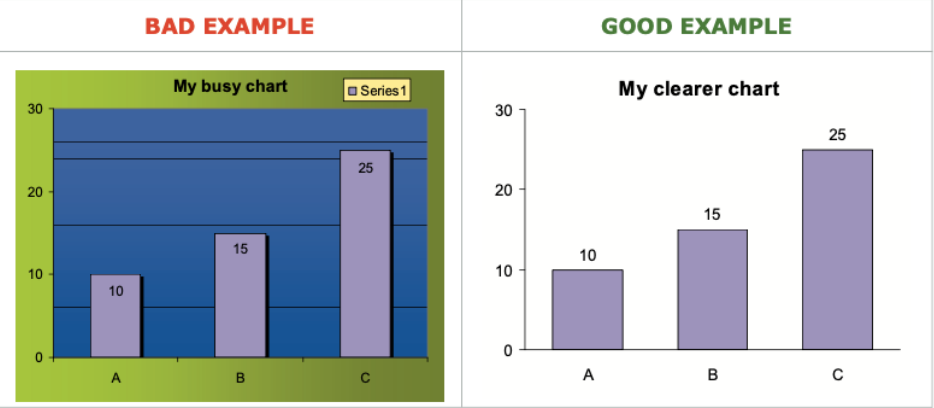
\includegraphics[keepaspectratio]{images/image2.png}}}

\begin{itemize}
\tightlist
\item
  {Istogramma}{: rappresentazione grafica di una distribuzione di una
  variabile numerica. }{Asse X: }{intervalli}{~}{invece }{Asse Y:
  }{frequenza}{.}
\end{itemize}

{\pandocbounded{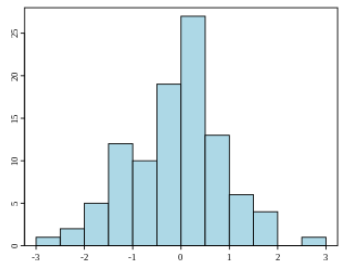
\includegraphics[keepaspectratio]{images/image5.png}}}

\begin{itemize}
\tightlist
\item
  {Grafico a torta}{: ~usato per rappresentazioni di variabili
  quantitative misurate su classi di categorie, circolare per evitare un
  ordine, ha il difetto che }{la dimensione delle slice non è un
  facilmente leggibile}{. }{NON}{~è la scelta migliore.}
\end{itemize}

{}

\begin{itemize}
\tightlist
\item
  {Treemap}{: visualizza i dati gerarchici come un insieme di rettangoli
  annidati.}
\end{itemize}

{\pandocbounded{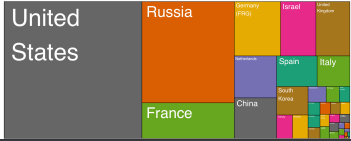
\includegraphics[keepaspectratio]{images/image12.png}}}

\begin{itemize}
\tightlist
\item
  {Area chart}{: descrivono i cambiamenti delle variabili nel tempo}
\end{itemize}

{\pandocbounded{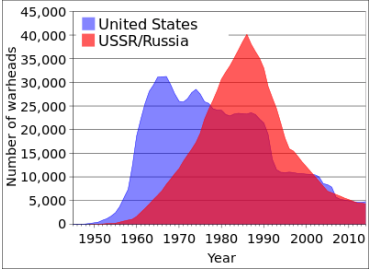
\includegraphics[keepaspectratio]{images/image11.png}}}

\begin{itemize}
\tightlist
\item
  {Stacked area chart}{: }
\end{itemize}

{\pandocbounded{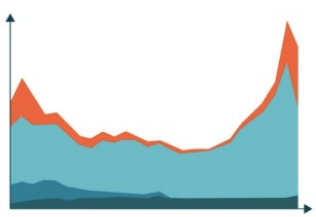
\includegraphics[keepaspectratio]{images/image4.png}}}

\begin{itemize}
\tightlist
\item
  {Line chart}{: utilizzati per rappresentare i dati delle serie
  temporali. È adatto a mostrare dati che cambiano in modo continuo.}
\end{itemize}

{\pandocbounded{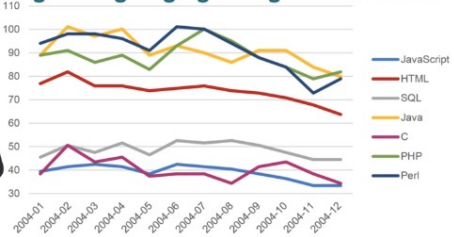
\includegraphics[keepaspectratio]{images/image14.png}}}

\begin{itemize}
\tightlist
\item
  {Scatter plot}{: due variabili di un dataset sono riportate su uno
  spazio cartesiano, dati visualizzati tramite una collezione di punti.}
\item
  {Bubble chart}{: tipo di grafico in cui ogni entità rappresentata è
  definita in termini di tre parametri numerici distinti. }
\item
  {Choropleth map}{: usano i colori per rappresentare quantità e qualità
  di una certa area geografica i cui confini sono prestabiliti.}
\item
  {Dot maps}{: usano una stessa forma per rappresentare ogni singola
  unità di dati. Il risultato visivo è che le zone con maggiore densità
  risultano ricoperte da una quantità maggiore di punti.}
\end{itemize}

{}

\section{\texorpdfstring{{D3.js}}{D3.js}}\label{h.v8q9ek1s8rk1}

{D3.js (Data-Driven Documents) è una libreria Javascript per produrre
visualizzazioni di dati dinamiche e interattive nei browser,
estremamente veloce e supporta comportamenti dinamici.}

{}

{}

{Gamification}

{``Gamification'' is the use of game design elements in non-game
contexts.}

{}

{}

\end{document}
